\documentclass[11pt]{article}
\usepackage{style}
\usepackage{MyNotations}
\begin{document}
\section{Pattern formation and Swift-Hohenberg model}
The first quantitative experiments and studies of pattern formation due to convection can be traced back to \emph{Henri Bérnard} \parencite{benardtourbillonscellulaires1901}. He studied the stability of a thin fluid layer open to air and submitted to a vertical temperature gradient. He accurately determined periodicity of the hexagonal pattern, as illustrated in \cref{fig:bernard}. After that, Lord Rayleigh \parencite{rayleighLIXconvection1916} proposed a theory based on a feedback coupling due to buoyancy in which a hot fluid particle hotter than its environment encounters ever colder fluid as it rises, which leads to the instability, and lead to the generation of convective currents. This instability later known as \emph{Rayleigh-Bérnard} instability was a a subject of several studies, namely the inclusion of surface tension effect.
\begin{figure}[H]
    \centering
    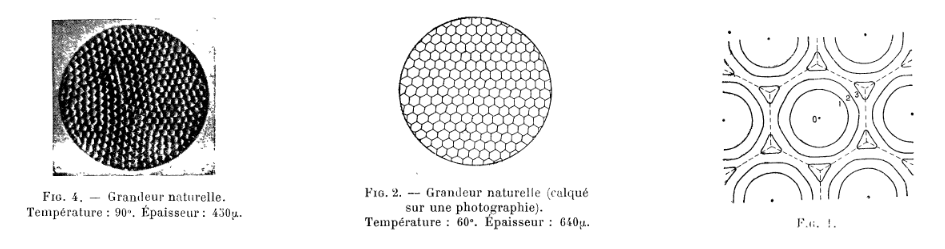
\includegraphics[width=0.8\textwidth]{imgs/pfc/bernard.png}
    \caption{Convection cells in \emph{Rayleigh-Bérnard} instability, from \parencite{benardtourbillonscellulaires1901}}\label{fig:bernard}
\end{figure}
One of its main features is that \emph{Rayleigh-Bérnard} convection exhibits well-ordered structure but that are formed under non-equilibrium conditions, (in contrast to crystalline materials). Fundamental questions concern the processes underlying the determination of the wavelength, and about the onset of the instability and how it is related to thermal fluctuations. \emph{Swift} and \emph{Hohenberg}, in 1977, proposed a model based on hydrodynamic fluctuations in order to study to what extent the non-equilibrium transition from a uniform to non uniform convecting state was similar to an equilibrium phase transition \parencite{swiftHydrodynamicfluctuations1977}. Their model was also aimed at understanding the effect of thermal fluctuations on this convective instability. They introduce order parameter $\psi(\vecc{x},t)$ which is meant to represent the vertical velocity of temperature fluctuation at the mid plane of the convective cell. The \emph{Swift-Hohenberg} model gives the evolution equation of $\psi$ as:
\begin{equation}
    \tau_0 \frac{\partial \psi}{\partial t} = \left[ \epsilon - \frac{\xi_0^2}{4q_c^2} \left( \nabla^2 + q_c^2 \right)^2 \right] \psi - g(\text{Pr}) q_c^2 \psi^3
\end{equation}
Where, we mainly highlight the fact that $\epsilon$ is the deviation of \emph{Rayleigh} number from its critical value. The previous equation can be rescaled to the following, classical form:
\begin{equation}
    \frac{\partial \psi}{\partial t} = \left[ \epsilon - \left( \nabla^2 + q_0^2 \right)^2 \right] \psi -  \psi^3
\end{equation}
\subsection{Special case : 1-d SH model}
One can gain much physical insight on the previous equation if we limit ourselves to the 1 dimensional case:
\begin{equation}
    \frac{\partial \psi}{\partial t} = \left[ \epsilon - \left( \partial_x^2 + q_0^2 \right)^2 \right] \psi -  \psi^3
\end{equation}
It it obvious that the homogeneous field $\psi_h=0$ is a solution of the 1-D \emph{Swift-Hohenberg} equation. In order to investigate wether this homogeneous solution, is stable as we vary the parameter $\epsilon$. We would like to determine the critical value $\epsilon_c$ when the state $\psi_h=0$ becomes linearly unstable, i.e. when the magnitude of an arbitrary infinitesimal perturbation $\delta\psi$ begins to grow exponentially in time.\\


Let's consider a perturbed field $\psi = \psi_h+\delta \psi$. At the first order in $\delta \psi$, neglecting higher powers, we find that it satisfies:
\begin{equation}\label{eq:lineardeltapsi_de}
    \partial_t \delta \psi = \left(\epsilon - q_0^4-\partial_x^4-2q_0^2\partial_x^2\right ) \delta \psi
\end{equation}
This linear differential equations admits a particular solution in the form of :
\begin{equation}
    \delta \psi(x,t)= A e^{\sigma t}e^{\alpha x}
\end{equation}
Replacing in the previous equation, one finds that:
\begin{equation}
    \sigma = \epsilon -(\alpha^2+q_0^2)^2
\end{equation}
If the domain is spatial infinite then $x$ can go to $\pm \infty$, in that case, we necessarily must have $\alpha \in i \mathbb{R}$ is a purely imaginary number, because if not then $\delta\psi$ is not a small perturbation (at least at $t=0$).\\ If the domain is periodic over length $L$, then one must have $\alpha L= (2 \pi m) $ for $m \in \mathbb{Z}$. So that, in any case, we write $\alpha = i q \in i \mathbb{R}$, with $q \in \mathbb{R}$. Finally, we get:
\begin{equation}
    \sigma(q) = \epsilon -(-q^2+q_0^2)^2
\end{equation}
Due to the linear nature of the differential equation \cref{eq:lineardeltapsi_de}, a general solution can be written as :
\begin{equation}
    \delta\psi(x,t)= \int_{-\infty}^{+\infty} A_q e^{\sigma(q) t} e^{iqx} \, dq
\end{equation}
If $\epsilon<0$, then $\sigma(q) <0 \, \forall \,  q$, meaning that all perturbations $\delta \psi$ decay exponentially in time $t\rightarrow \infty$. This translates to the fact that the homogeneous state $\psi_h=0$ is linearly stable. However, as soon, as $\epsilon=\epsilon_c=0$, stability is lost for the mode $q=\pm q_0$, and as soon as $\epsilon>0$, ever slightly, the domain where $\sigma(q)>0$ gets bigger and Fourier modes with vector close to $q_0$ will exponentially grow in time. This suggest, the onset of pattern formation and predicts the formation of some cellular structure with a characteristic wavelength $2\pi/q_0$.
\subsection{Amplitude equation}
We previously saw that the unstable state is associated with a wave vector $q_0$ (being the first wave number to grow at the onset of instability $\epsilon=0$). However, in reality, the system cannot be tuned precisely to this case, thus, at the onset of instability $\epsilon<<1$, a finite interval, close to $q_0$ will have an exponential growth in time ($\sigma(q)>0$). What happens as all these modes grow can be investigated using the Amplitude equation formalism and be easily understood by analogy to the beating and modulation of two cosine functions with close wave numbers.
The superposition of oscillations with similar frequencies leads to a “beating” in the overall amplitude. For a pattern forming system, this means that the
strength of the pattern (the amplitude) varies much more slowly than
the pattern itself.
\begin{figure}[H]
    \centering
    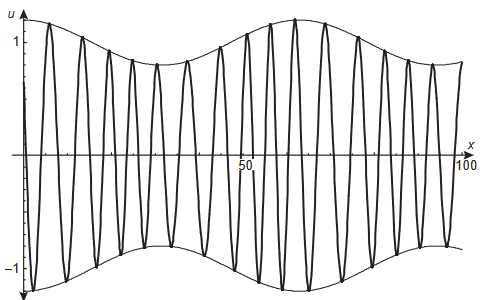
\includegraphics[width=0.4\textwidth]{imgs/pfc/modulation.png}
    \caption{Example of a parametric plot ($\sin (x), \cos(x), x$)}\label{fig:modulation}
\end{figure}
Near onset $\epsilon<<1$, we separate fast and slow variables of space and time by introducing:
\begin{equation}
    X = \epsilon^{1/2} x, \quad Y = \epsilon^{1/4} y, \quad T = \epsilon t
\end{equation}
Expanding, $\psi =\epsilon^{1/2} \psi_0+\epsilon \psi_1+\dots $, at the lowest order we must satisfy:
\begin{equation}
    \left( \partial_x^2 + q_0^2 \right)^2 \psi_0 = 0 \quad \Rightarrow \quad \psi
    _0(x,t)=A(X,Y,T) e^{iq_0x}+\cdots
\end{equation}
Solvability conditions lead to :
\begin{equation}
    \tau_0\partial_t A = \epsilon A +\xi_0 \left[ \partial_x-(i/2q_0) \partial_y^2\right]^2A-g_0 |A|^2 A
\end{equation}
Which is the amplitude equation that describes the evolution in space and time of the slow modulations of the base solution $\psi_0$.  This allows us to see the \emph{Ginzburg-Landau}XX equation as amplitude equation for the single Swift–Hohenberg equation XX.
\subsection{The variational formulation of Swift-Hohenberg equation}
One can observe that \emph{Swift-Hohenberg} equation has a variational structure. It means that it possesses a \emph{Lyapunov} functional $\mathcal{F}$, known as $SH$ free energy:
\begin{equation}
    \partial_t = \psi = - \frac{\delta \mathcal{F}}{ \delta \psi} \quad \text{With} \quad \mathcal{F}[\psi] = \int \vecc{dx} f(\psi,\nabla^2\psi) = \int \vecc{dx} \left[ - \frac{\epsilon}{2} \psi ^2 + \frac{1}{2}\left( \nabla^2+q_0^2\right)^2 \psi^2  + \frac{1}{4} \psi^4 \right]
\end{equation}
With $f$ being a free energy density. The time derivative of the free energy can be written as:
\begin{equation}
    \frac{d \mathcal{F}}{dt} =\int \vecc{dx} \left\lbrace-\epsilon \dot \psi \psi+\left[  \left( \nabla^2+q_0^2\right)^2 \psi \right] \dot \psi + \psi^3 \dot \psi \right\rbrace = - \int \left( \frac{\partial \psi}{\partial t}\right)^2 \vecc{dx} \leq 0
\end{equation}
Hence, $\mathcal{F}$ is a decreasing "energy" through the evolution of the system.  The dynamics is “downhill” and is sometimes called gradient flow. In addition, the final states can be obtained by finding minima of $\mathcal{F}$.

\subsection{The concept of order parameter}
\emph{Rayleigh-Bénard} convection patterns are just one example of non-equilibrium pattern formation, a phenomenon seen across multiple and diverse systems. Experimental and theoretical studies suggest that similar pattern formation processes occur universally across these systems, indicating that spontaneous pattern formation in non-equilibrium systems can be described by the same mathematical tools, regardless of their specific characteristics.\\
This universality can be understood through the concept of \emph{Order parameter}. Analysis shows that order parameters, governed by nonlinear partial differential equations, dictate the spatial and temporal evolution of patterns in various systems. Remarkably, systems as different as reaction-diffusion models and convection experiments exhibit the same underlying order parameter dynamics. This concept is particularly valid for systems near instabilities, where patterns emerge predictably from the system's fundamental mathematical structure. Consider some arbitrary pattern formation system described by a state vector $\vecc{q}(\vecc r,t)$, it obeys some partial differential equation:
\begin{equation}
    \partial_t \vecc q = \Theta [\vecc q(\vecc r,t)]
\end{equation}
Where $\Theta$ is some differential operator. The long term behavior of $\vecc q(\vecc r,t)$, can be captured by an order parameter $\psi$, linked with $\vecc q$ and it can be directly related to some easily observable physical quantity. The validity of the order parameter concept can be proved for systems close to instabilities, where the system’s behavior changes qualitatively. The order parameter in the case of \emph{Rayleigh-Bérnard} convection is the temperature field ( or vertical velocity), it is the magnetization vector in the case of ferromagnets, or even an indicator function of the different phases in \emph{Cahn-Hilliard} model, or damaged/undamaged materials in Gradient-damage facture models. An order parameter equation generally reads:
\begin{equation}
    \partial_t \psi = h [\psi(\vecc r,t)]
\end{equation}

\subsection{Topological defects in SH and PFC models}
The equilibrium and dynamics of defects, in a small scale, plays in important role in the studies of the evolution of complex systems at different scales \parencite{anghelutaAnisotropicvelocity2012}. Their statistical properties have a huge impact on the evolution of system, examples are given in quenching dynamics during phase ordering kinetics, defects in convection pattern, and dislocation dynamics in crystal plasticity. The emergence of topological defects is a common phenomena is systems supporting a continuous symmetry that is spontaneously broken during non-equilibrium phase transitions \parencite{anghelutaAnisotropicvelocity2012}. \\
The topological theory of defects, as formalized by \parencite{mermintopologicaltheory1979}, gives an elegant and precise language to understand the formation of defects. In fact, defects aries whenever the order parameter manifold is not simply connected, i.e it has a non trivial fundamental group $\pi_0$ \parencite{pismenVorticesNonlinear1999}. The equilibrium properties of defects and their link with topological properties was heavily studied in \parencite{pismenVorticesNonlinear1999}. The formulation and evolution of topological defects is formulated, typically, through the complex \emph{Ginzburg-Landau} equation, where defect are described as phase singularities (The phase evolving in the circle $\mathcal{S}^1$, with non trivial homotopy group $\pi_0\simeq  \mathbb{Z}$).

The impact of dislocations on melting of solids was extensively studies in the 80's. The order liquid-crystal films was studied in \parencite{tonerSmecticcholesteric1981} \parencite{nelsonBondorientationalorder1981} while focusing the effect of dislocations and thermal fluctuations. In the same year, \emph{Siggia} and \emph{Zippelius} studied the dynamics of defects in \emph{Rayleigh-Bérnard} convection using the gradient flow of the complex amplitude \parencite{siggiaDynamicsdefects1981}. Later one, the \emph{Swift-Hohenberg} model was used to study motion of isolated dislocations in Rayleigh-bernard roll structure \parencite{shiwaDislocationmotion1986}. \emph{Halperin} introduced an analytical method of locating and tracking defects using Dirac's delta function $\delta$ \parencite{Halperin1981}. Further more,  this method was extended by \emph{Mazenko} \parencite{mazenkoOrderingkinetics1998a} to excplicitly determine the velocities of topological defects. The idea behind the formalism is that in the "real space", let's say of dimension $d$, topological defects of a $d-$dimensional order parameter given as a vector field $\bm\psi(r)=\left\lbrace \psi_\alpha(r)\right\rbrace_{1\leq\alpha\leq n}$, are located at the zeros of the vector field. In fact, the "orientation" $\bm \psi / ||\bm \psi||$, is well defined everywhere iff $\psi \neq 0$. So that the defects, i.e points where no orientation can be determined, are located by the zeros of $\bm \psi$; in other words, whenever $\delta(\bm \psi) =1$. This definition holds in the space of $\bm \psi$, also known as the order parameter's manifold. In order to locate defects in the real space, we introduce the jacobian $\mathcal{D}$ of the variable transformation from the real space position $\vec{\bm r}$ to the order parameter manifold $\bm \psi$. Thus, we define a defect density $\rho_d(\bm r)$\parencite{Halperin1981}, in the real space, as :
\begin{equation}
    \rho_d(\bm r,t) = \delta(\psi) \mathcal{D}(\bm r,t)=\sum_i q_i \delta(\bm r -\bm{r_i})
\end{equation}
This formula establishes the link between the distribution of defects located at position $\bm{r_i}$ having a topological charge $q_i = \mathcal{D}(\bm{r_i},t)/||\mathcal{D}(\bm{r_i},t)||$ to the zeros of the $d-$dimensional order parameter $\psi$. Note that when  writing $\rho_d(\bm r,t) = \delta(\psi) \mathcal{D}(\bm r,t)$, the time dependence is only in $\mathcal{D}$, that's is to say the order parameter's manifold isn't changing it's the map from real space to it that's changing and carrying the time evolution information of the topological charges. In order to illustrate the previous equation, let's specialize for example to the case where $d=2$ and the order parameter is complex number, let's say $\psi = (\psi_1,\psi_2)$ i.e $n=2$. The orientation (phase) of $\psi$ vanishes only in a set of separated point $\vec{r_i}$. The jacobian $\mathcal{D}(r)$ is a scalar quantity \parencite{anghelutaAnisotropicvelocity2012}:
\begin{equation}
    \mathcal{D}(r)= \begin{vmatrix}
        \partial_x\psi_1 & \partial_y\psi_1\\ 
        \partial_x\psi_2 & \partial_y\psi_2\\
   \end{vmatrix} = \partial_x\psi_1 \partial_y\psi_2 - \partial_y\psi_1\partial_x\psi_2 = \frac{1}{2i} \left\lbrace \partial_x \psi^* \partial_y \psi -\partial_x \psi \partial_y \psi^*\right\rbrace
\end{equation}
The case where $d>n$ is more subtle to treat since jacobian of the transformation $\vec{r}\mapsto \psi(\vec{r})$ is not a square matrix and a determinant cannot computed. The orientation of the field can vanish on spaces *\marginpar{introduce codimension} of higher dimensions. The example of $d=n+1$ was treated in \parencite{Halperin1981} and further detailed in \parencite{mazenkoVelocitydistribution1999} to explicity compute velocities. In this case defects are lines, with line density given, in terms of its components, by:
\begin{equation}
    \rho_\alpha =\delta(\psi)\mathcal D_\alpha(r) \quad \text{with} \quad \mathcal{D}_\alpha = \frac{1}{n!} \epsilon_{\alpha i_2\dots i_d}\epsilon_{j_1j_2\dots j_n} \partial_{i_2} \psi_{j_1}\partial_{i_3} \psi_{j_2} \dots \partial_{i_d} \psi_{j_n} \quad , \quad 1\leq\alpha\leq d
\end{equation}
with $\epsilon_{\alpha i_2\dots i_d}$ being the fully anti-symmetric \emph{Levi-Civita} tensor of order $d$. The rather cumbersome notation of the previous equation can be made simple in the case where $d=3$ and $n=2$. 
\begin{equation}
    {D}_\alpha = \frac{1}{2} \epsilon_{\alpha jk}\epsilon_{lm} \partial_{j} \psi_{l}\partial_{k} \psi_{m} = \frac{1}{2} \epsilon_{\alpha jk} \left[ \partial_j \psi_1 \partial_k \psi_2 - \partial_j \psi_2 \partial_k \psi_1 \right] =   \epsilon_{\alpha jk}\left(\partial_j \psi_1 \partial_k \psi_2\right)
\end{equation}
Because $\epsilon_{\alpha jk} = -\epsilon_{\alpha kj}$. So that the $i$-component of the tangent vector to the defect line at point $\bm r$ are given by $\rho_i(\bm r) = \delta(\psi ) \epsilon_{i jk}\left(\partial_j \psi_1 \partial_k \psi_2\right)$. In addition, \emph{Mazenko} \parencite{mazenkoVortexVelocities1997} derived an explicit relation giving the velocity of defects. Using the fact that the determinant is a conserved invariant satisfying a continuity equation, with a current $\bm{\mathcal{J}}^\psi$ we write, in the case of a point defect ($n=d=2$):
\begin{equation}
    \partial_t \mathcal{D} +\nabla \cdot \bm{\mathcal{J}}^\psi = 0 \quad \text{with} \quad \mathcal{J}^\psi_\alpha = -\frac{i \epsilon_{\alpha\beta}}{2}\left(\dot \psi \partial_\beta \psi^*-\dot \psi^*\partial_\beta \psi\right)
\end{equation}
By taking the time derivative of $\rho(r)=\delta(\psi)\mathcal{D}(r)$ we get:
\begin{equation}
    \begin{aligned}
        \partial_t\rho &= \partial_t(\delta( \psi))\mathcal{D}+ \delta(\psi) \partial_t \mathcal{D}\\
        &=\frac{\partial \delta}{\partial \psi} \dot{\psi}\mathcal{D}+\delta(\psi) \partial_t \mathcal{D}\\
        &=\frac{\partial \delta}{\partial \psi} \dot{\psi}\mathcal{D}-\delta(\psi) \nabla \cdot \mathcal{J}^\psi \quad (\text{by the continuity law of } \mathcal{D})\\
    \end{aligned} 
\end{equation}
An algebraic manipulation allows us to re-write $\dot{\psi}\mathcal{D}$. In fact:
\begin{equation}
    \renewcommand\arraystretch{1.8}
    \mathcal{J}^\psi\cdot \nabla\psi = \begin{bmatrix}
        -\cfrac{i}{2} \left(\dot \psi \partial_y \psi^*-\dot \psi^*\partial_y \psi\right) \\
        \cfrac{i}{2} \left(\dot \psi \partial_x \psi^*-\dot \psi^*\partial_x \psi\right)
    \end{bmatrix} \cdot \begin{bmatrix}
        \partial_x \psi \\
            \partial_y \psi
    \end{bmatrix} = \frac{i}{2} \dot \psi \left( \partial_x\psi^*\partial_y \psi-\partial_x\psi\partial_y \psi^*\right) = -\dot \psi \mathcal{D}
\end{equation}
Replacing in the time derivative of the density $\rho$:
\begin{equation}
    \partial_t \rho = \frac{\partial \delta}{\partial \psi} \dot{\psi}\mathcal{D}-\delta(\psi) \nabla \cdot \mathcal{J}^\psi= -\frac{\partial \delta}{\partial \psi} \mathcal{J}^\psi\cdot \nabla\psi-\delta(\psi) \nabla \cdot \mathcal{J}^\psi = - \nabla\cdot(\delta(\psi)  \mathcal{J}^\psi) = - \nabla\cdot(\rho \frac{ \mathcal{J}^\psi}{\mathcal{D}})
\end{equation}
By identification with the classical form of density conservation ($\partial_t \rho + \nabla \cdot(\rho v) =0$), we define point defect velocity \parencite{mazenkoVortexVelocities1997} :
\begin{equation}
    \bm{v}= \frac{1}{\mathcal{D}} \bm{\mathcal{J}}^{\psi}
\end{equation}
The previous result yields a way of determining the velocity of point defects directly from the complex order parameter $\psi$. This result can be easily generalized to higher dimensions, as extensively detailed in \parencite{mazenkoVelocitydistribution1999}. Within this work, we limit ourselves to case where $n=2,d=3$. The velocity a dislocation curve is given by:
\begin{equation}
    \vec{v} = \frac{1}{2 ||\vec{\mathcal{D}}||^2}\left( \vec{\mathcal{D}} \times (\dot \psi^* \nabla \psi - \dot \psi \nabla \psi^*)\right)
\end{equation}
Where $\vec{\mathcal{D}} = (\mathcal{D}_i)$, the vector of determinants as previously defined, because the jacobian of the transformation is not a square matrix and in this case the current is second order tensor $\mathcal{J}_{ij}^\psi$ \parencite{mazenkoVelocitydistribution1999}.\\ 
This paradigm herein introduced applies only to multi-dimensional order parameters $\bm\psi(r)=\left\lbrace \psi_\alpha(r)\right\rbrace_{1\leq\alpha\leq n}$. It was extended in \parencite{skaugenDislocationdynamics2018}\parencite{skogvollphasefield2022} to study the motion of dislocations in defect crystal with PFC-model using the amplitude expansion as we shall next. In 2023, a unified field theory generalizing the work of \emph{Mazenko} was proposed  \parencite{skogvollunifiedfield2023} in order to describe defects and non-linear fast excitations in different systems : Bose-Einstein condensates, active nematics and crystal lattices.
\section{Phase Field crystal model}
\subsection{Introduction}
The Phase Field Crystal (PFC) model was introduced in 2002 by \emph{Elder} and \emph{Grant} \parencite{elderModelingElasticity2002} in order to include elasticity in crystal growth. The Swift-Hohenberg free energy was used and they argued that the factor $(\nabla^2+q_0^2)$ was the simplest way the include peaks in the resulting structure at $q_0$ wavelength, which emulates the emergence of periodic crystal structure. Crystalline pattern was the key ingredient to include elasticity in the crystal growth model \parencite{elderModelingelastic2004}. In the PFC model, the scalar field $\psi$ is a local average density and hence it's integral over the domain was meant to remain conserved (mass conservation). Thus, using \emph{Swift-Hohenberg} functional $\mathcal{F}_{sh}[\psi]$, the phase field crystal model uses conserved dynamics to derive the evolution equation of $\psi$:
\begin{equation}
    \partial_t \psi =  \nabla \cdot \left(\Gamma \nabla \frac{\delta \mathcal{F}_{sh}}{\delta \psi}\right) \quad \text{with} \quad \mathcal{F}_{sh}[\psi] = \int \vecc{dx} \left[ - \frac{\epsilon}{2} \psi ^2 + \frac{1}{2}\left( \nabla^2+q_0^2\right)^2 \psi^2  + \frac{1}{4} \psi^4 \right]
\end{equation}
This functional is minimized by constant (liquid state), strip state and hexagonal (triangular state) which can be understood as crystalline state. Despite its simplicity, the PFC model gives respectable descriptions of elasticity, since it was used to derive elastic constants by calculating the change of energy under some applied deformation \autocite{elderModelingElasticity2002}, It was also used to compute yield stress and model softening \parencite{elderModelingelastic2004}. In addition, it reproduces both \emph{Read-Shockley} grain boundary energies and \emph{Matthews} and \emph{Blakeslee} misfit dislocation behavior during epitaxy \parencite{elderModelingElasticity2002}, and can accurately model liquid-phase epitaxial growth \parencite{elderModelingelastic2004}. The PFC model has been used in numeral mechanical studies included fracture propagation \parencite{elderModelingElasticity2002}, plasticity avalanche \parencite{chanPlasticityDislocation2010}, and edge dislocation dynamics \parencite{elderPhasefieldcrystal2007}. \\


Although originally phenomenologically motivated, the PFC model had been derived from classical density functional theory \parencite{archerDerivingphase2019} \parencite{wuPhasefieldcrystal2007}. To go into details, DFT describes a system of $N$ interacting particles at positions $\vecc{r}_i$ by an average one variable particle density $\rho(\vecc{r})$ (inspired by pioneering work of \emph{Hohenberg} and \emph{Kohn} in the context of Quantum mechanics in order to provide approximate solutions to the multi-body \emph{Shrödinger} equation). In the ne canonical ensemble, the average density is simply given by an ensemble average $\langle \cdot \rangle$:
\begin{equation}
    \rho(\vecc{r})= \left\langle \sum_{i=0}^{N} \delta(r-r_i) \right\rangle
\end{equation}
According to the \emph{Hohenberg-Kohn} principle, there exist a free energy functional $\Omega[\rho]$ minimized at equilibrium. This functional is linked to Helmholtz free energy $\mathcal{F}$ by a simple legendre transformation:
\begin{equation}
    \Omega[\rho,\mu,T] = \mathcal{F}[\rho,T] - \mu \underbrace{\int \rho (r) dr } = \mathcal{F}[\rho,T] - \mu N
\end{equation} 
In classical DFT calculations, Helmholtz free energy is decomposed into two main contribution, in the absence of any external field, so that we write:
\begin{equation}
    \mathcal{F}[T,\rho] =\mathcal{F}_{id}[T,\rho]+\mathcal{F}_{ex}[T,\rho]
\end{equation}
The functional $\mathcal{F}_{id}[T,\rho]= k_BT \int \rho(r) \left( \ln(\Lambda^3 \rho(r))-1\right) \, dr$ corresponds to  the free energy of an ideal gas with $k_B$ being Boltzmann's constant and  $\Lambda = h/\sqrt{m=2mk_BT}$ de Broglie's wavelength. The second term $\mathcal{F}_{ex}[T,\rho]$ corresponds to the excess free energy (deviation from ideal gas) due to all correlations from all interactions between particles. This functional is not known and is only approximated. For that, we perform a taylor expansion around a uniform reference state $\rho_{ref}$. If we denote $\Delta \rho = \rho(r)-\rho_{ref}$, Taylor expanding yields:
\begin{equation}
    \mathcal{F}_{\text{exc}}[T, \rho] = \mathcal{F}^{(0)}_{\text{exc}}[\rho_{\text{ref}}] + \sum_{n=1}^{\infty} \int d\mathbf{r}_1 \dots \int d\mathbf{r}_n \frac{1}{n!} \frac{\delta^n \mathcal{F}_{\text{exc}}[T, \rho(\mathbf{r})]}{\delta \rho(\mathbf{r}_1) \dots \delta \rho(\mathbf{r}_n)} \bigg|_{\rho_{\text{ref}}} \prod_{i=1}^{n} \Delta \rho(\mathbf{r}_i)
\end{equation}

Since we are interested in the derivatives of $\mathcal{F}$, we can neglect the $0$-th order term and the first order term too, who turns one to be a constant due to the isotropy of the bulk fluid. If We truncate the previous equation at its second order, we write:
\begin{equation}
    \begin{aligned}
        \mathcal{F}_{\text{exc}}[T, \rho] &= \frac{1}{2!} \iint \frac{\delta^2 \mathcal{F}_{\text{exc}}[T, \rho(\mathbf{r})]}{\delta \rho(\mathbf{r}_1) \delta \rho(\mathbf{r}_2)} \bigg|_{\rho_{\text{ref}}} \Delta \rho(\mathbf{r}_1)\Delta \rho(\mathbf{r}_2) \, d\mathbf{r}_1 \, d\mathbf{r}_2\\
        &= - \frac{k_B T}{2} \iint C_2(\mathbf{r}_1-\mathbf{r}_2) \Delta \rho(\mathbf{r}_1)\Delta \rho(\mathbf{r}_2) \, d\mathbf{r}_1 \, d\mathbf{r}_2
    \end{aligned}
\end{equation}
Where $C_2(\mathbf{r}_1-\mathbf{r}_2)$ is the pair correlation function, and is the key ingredient to fine tuning the phase field crystal to procuce some desired phase diagrams as we shall see next. With the basis of DFT established, the dynamics are described by the central equation of \emph{dynamical density functional theory} (\textbf{DDFT}), the conserved dissipative dynamics is given by:
\begin{equation}
    \partial_t \rho(\mathbf{r},t) = \nabla \cdot \left[ (k_BT)^{-1}M(\rho) \nabla \frac{\delta \mathcal{F}}{\delta \rho}\right]
\end{equation}
With $M(\rho)$ being the mobility.\\


The model originally introduced, in 2002, is unfortunately only able to produce uniform, stripes and hexagonal (triangular states) and a corresponding phase diagram was produced \parencite{elderModelingelastic2004}. This limitation was quickly noticed, and a minor modification by Alain Karma was considered in order to produce BCC structures in 2D \parencite{wuPhasefieldcrystal2007}. Shorty after, in 2007, the 2D phase diagram (with BCC structures) was extended to 3D \parencite{jaatinenExtendedphase2010}.\\
From a classical density functional theory,  it was possible to predict both fcc and hcp structures, but this result has never been successfully reproduced in the PFC community, because of the liquid correlation function $C_2$ used, that does not seem to contain enough information to determine the solid state crystal structure. In 2011, It was shown that the excess free energy, can be constructured to create an energy minimum for a desired periodic structure \parencite{greenwoodPhasefieldcrystalmethodology2011}, so that progress has been made in the PFC community by considering phenomenological forms for the Fourier transform of the two-point correlation function $\hat C_2$, carefully designed to stabilize a target structure: triangular and square lattices in 2D, and bcc, fcc, hcp, and sc lattices in 3D. Then, Following the same direction, it was shown in 2013 that the PFC model can be tuned to reproduce all five bravais lattices in 2D \parencite{mkhontaExploringComplex2013}.

\subsection{Time scale in PFC}
The fundamental time scale involved in phase field crystal is the diffusion time \parencite{elderModelingelastic2004}, because the model averages over rapid fluctuations in time to give a time scale of evolution on the order of diffusion rather than atomic vibration. To see that, consider a perfect equilibrium configuration $\psi_{eq}$ of the original PFC model. Then, suppose that one particle is removed to create a vacancy in the lattice. Atomic vibrations will cause neighboring atom to hop into the vacancy so that the this defect will diffuse throughout the lattice. However, the vibration are integrated out in the PFC model and the all that is left is diffusion. In this sense, and from a phase field point of view, the density at the missing spot will gradually increase as the density at neighboring sites slowly decreases.\\


However, there are many phenomena, of important physical interest, that exist between the time scale of atomic vibration and the diffusive time scale \parencite{stefanovicPhaseFieldCrystals2006}. But due to the dissipative dynamics of diffusing the scalar field, PFC model cannot model for example elastic interactions or fast dynamics \parencite{heinonenConsistentHydrodynamics2016}. In a first attempt, \emph{Stefanovic} proposed a \emph{modified phase field crystal} (\textbf{MPFC}) model able to transmit short wavelength density fluctuation up to a time scale $t_w$ after which the evolution continues diffusely \parencite{stefanovicPhaseFieldCrystals2006}, but failed to describe large scale vibrations and couldn't reproduce correct phonon dispersion curves as noticed by \parencite{majaniemiDissipativephenomena2007},\parencite{majaniemiFirstprinciplesphenomenological2008}. The MPFC relies on including a second derivative, to add a wave-mode, in the time evolution equation of the scalar field $\psi$, it reads :
\begin{equation}
    \frac{\partial ^2\psi}{\partial t^2} + \beta \frac{\partial \psi}{\partial t} = \alpha^2 \nabla^2 \frac{\delta \mathcal{F}}{\delta \psi}
\end{equation}
In most up-to-date research, the phase field $\psi$ is interpreted as a mass density, so that lattice distortion and mass variations are described by the same scalar, that evolves diffusively which is not physical. These two quantities, i.e mass and displacement should be considered independently \parencite{acharyaElasticityphase2022}. This difficulty, along with including dissipation at a macroscopic scale remained unclear in challenging. \emph{Heinonen} in 2016, formulated a complete hydrodynamic-PFC model which couples fast dynamics to dissipative processes on a mesoscopic length scale \parencite{heinonenConsistentHydrodynamics2016}. He introduced a mesoscopic mass velocity $v$, and mass density $\rho$. The mass displacement, and lattice displacement are now subject to independent variations. Evolution equations were obtained by coarse graining \parencite{athreyaRenormalizationgrouptheory2006} the mass density and velocity fields by using the amplitude expansion framework and adding a dissipative \emph{Navier-stokes} term. This model accurately describes fast dynamics but can be computationally expansive, especially if the mechanical relaxation happens several order of magnitudes faster than diffusion and plastic flows. Alternatively, an approach based on interpolation was proposed in \parencite{zhouMechanicalrelaxation2019}, in which the linear elastic displacement field was used to interpolate between grid points in order to ensure mechanical equilibrium but it was only valid for uniaxial loadings. A more recent work \parencite{skaugenSeparationElastic2018}, used the fact that the phase field crystal gives a good description of the incompatible part of mechanical stress so that it was supplmented by a smooth  displacement field $u^\delta$ to ensure mechanical equilibrium $\psi(\bm r) \rightarrow \psi(\bm r - \bm u ^\delta)$. This approach, later known as \textbf{MEqPFC}, was applied to the \emph{amplitude phase field crystal} \textbf{APFC} to give a better computational approach to large systems \parencite{salvalagliocoarsegrainedphasefield2020}.\\


Another path was the idea of scale separation using fourier filters as introduced in \parencite{tothNonlinearhydrodynamic2013}, so that the dissipation of velocity was handled in the long rage limit but this model, as originally proposed, lacked the classical dissipation of the PFC model. This was introduced, along with fourier filters in \parencite{podmaniczkyNucleationPostNucleation2021} as a phenomenological damping parameter.\\
More recently, \emph{Skogvoll} in 2022, suggested a consistent derivation of a coupling between PFC dynamics and a macroscopic velocity field \parencite{skogvollHydrodynamicphase2022}. The separation of scales is done by means of fourier filers, just like \parencite{tothNonlinearhydrodynamic2013}. Nonetheless, it is more versatile than the model suggested in \parencite{heinonenConsistentHydrodynamics2016} since it remains valid for large deformation too.

\subsection{Dislocation dynamics with the PFC model}
As previously seen, the phase field crystal model (PFC) was introduced as mesoscale description of crystalline solids. Since defects naturally emerge and evolve in the PFC model without any imposed rules, it was heavily used to study dislocations at the atomistic level \parencite{berryDiffusiveatomistic2006}\parencite{elderPhasefieldcrystal2007a}\parencite{chanPlasticityDislocation2010}. However, a mesoscale model that bridges the atomic description with the macroscale continuum theory of mechanics and crystal plasticity (induced by the motion of dislocations) was still lacking.\\
In 2018, a first attempt was proposed to develop a theoretical framework to study plastic flow (on a large scale) due to dislocation motion (on a small scale) \parencite{skaugenDislocationdynamics2018}. The authors derived the configurational elastic stress by analyzing variations in the free energy under weak distortions:
\begin{equation}
    \sigma_{ij}^\psi = [\partial_i \mathcal{L} \psi] \partial_j \psi - [\mathcal{L}\psi]\partial_{ij} \psi -f \delta_{ij}
\end{equation}
Furthermore, they then linked the classical Burgers vector density to field singularities using the \emph{Mazenko-Halperin} method \parencite{Halperin1981}\parencite{mazenkoVortexVelocities1997}. The phase-field crystal (PFC) model, which is based on the \emph{Swift-Hohenberg} framework, uses a smooth, non-singular scalar field for the order parameter $\psi$, which inherently limits its ability to capture defects. However, close to the bifurcation point, an amplitude expansion is applicable, allowing complex amplitudes $A_n$ to be used to identify defect locations (by tracking the zeros of $A_n$) and explicitly determine their velocities. Under specific assumptions, the authors also derived an expression that relates the velocity of dislocations to the average elastic stress (as determined from the phase field)\parencite{skaugenDislocationdynamics2018}. This expression aligns with the classical \emph{Peach-Koehler} force and provides an explicit form for the mobility coefficient. They validated their theory by examining the pure climb and pure glide of a dislocation dipole within a hexagonal lattice, observing that dislocations moved until they annihilated, which aligns with expected physical behavior. Furthermore, the authors compared the average elastic stress $\langle \sigma^{\psi}_{ij}\rangle$ obtained from the PFC model with classical elasticity solutions. They found good agreement between the two approaches, except within the dislocation core region. When comparing the tracked velocities to those predicted by the Peach-Koehler force, they observed a clear and significant discrepancy, which goes back to the fact that the mechanical information ($\sigma_{ij}^\psi$) encoded in the phase field is irrelevant. The model was evolving dislocations outside a mechanically equilibrated setting.\\


As long as the phase field $\psi$, that evolves diffusively, is interpreted as a mass density, mechanical equilibrium cannot be assured. Plastic motion is slow on the scale of lattice variation and happens at mechanical equilibrium. However, any non equilibrium deformation of $\psi$ will only evolve diffusively which is unphysical. An attempt at detaching mass motion and lattice distortion was then proposed in \parencite{skaugenSeparationElastic2018}, by explicitly accounting for the separation of elastic and plastic time scales. They retain the PFC model since it acts a reliable tool to locate and track defects, and they supplement it with a smooth distortion field $u^\delta$ to ensure mechanical equilibrium. In fact, the phase field only gives the incompatible part of the stress $\sigma^{\psi}_{ij}$ to which they add another smooth contribution to ensure that equilibrium is preserved.
\begin{equation}
    \sigma_{ij} = \sigma^{\psi}_{ij}+\sigma^{\delta}_{ij}=\sigma^{\psi}_{ij}+\lambda \delta_{ij}u_{kk}^\delta+2\mu u_{ij}^\delta 
\end{equation}
The smooth field $u^\delta$ has no impact on dislocation density (since the latter is defined as curl), and it is used to displace the field at each time step $\Delta t$ : $\psi(\bm r) \rightarrow \psi(\bm r + \bm u ^\delta)$. Conveniently, this additional field serves as straightforward way to implement boundary conditions when solving for $u^\delta$ using Airy's stress function $\chi$ in a more computationally performant than the penalty term $M(x,y)(\psi-\psi_{trac})^2$ classically used to apply axial strain introduced \parencite{stefanovicPhasefield2009}. As a benchmark of their mechanically equilibrated PFC theory \parencite{skaugenSeparationElastic2018}, the authors studied annihilation of a dislocation dipole in glide condition. The model gave a velocity that agrees with the classical theory, and regularized stresses that agreed with the linear elasticity solutions far for the core (the classical solution diverges in the core). This approach, known as \textbf{MEqPFC}, was also applied in the amplitude phase field crystal model for better computational approach in large systems \parencite{salvalagliocoarsegrainedphasefield2020}.
The fact that dislocations give rise to lattice incompatibilities and that the phase field $\psi$ is a good descriptor of the incompatible stress, it seems only natural to use the incompatible strain in order to study dislocation nucleation. Authors in \parencite{skogvollDislocationnucleation2021} introduced a incompatibility field $\eta^\psi$:
\begin{equation}
    \eta^{\psi} = \frac{1}{2\mu} \left( \epsilon_{ik} \epsilon_{jl} \partial_i \sigma_{kl}^{\psi} - \kappa \nabla^2 \sigma_{kk}^{\psi} \right).
\end{equation}
They showed that the incompatibility field can accurately be used to diagnose dislocation nucleation. In fact, the location of the maximum $\max \eta^\psi$ gives an indicator of where the nucleation dipole will appear and the symmetry of $\eta^\psi$ prior to nucleation yields the Burgers vector direction. Following this work, a full theory of the Kinematics of dislocation lines in three-dimensional anisotropic crystal solids was proposed in \parencite{skogvollphasefield2022}. The authors applied it to study dislocation loops and showed that the motion is driven by a Peach-Koehler like force and it gives stresses that agree with classical solutions in the far field. Even more recently, \emph{Skogvoll} \parencite{skogvollHydrodynamicphase2022} suggested a a complete and general coupling of hydrodynamics and phase field crystal able to couple the diffusive evolution of the scalar field with the fast dynamics of a macroscopic velocity field, using coarse-graining. It was shown that the resulting model is able to the evolve the PFC at mechanical equilibrium. The authors argued that the model is general an can used to study large deformations and dynamics since it captures elastic waves properly.
\section{Field dislocation mechanics and phase field crystal}
It was already pointed out before that the main shortcoming of the phase field crystal is that scalar field $\psi$ is interpreted as a mass density so that lattice and mass do not independent variations. Their evolution is bound the disspative diffusion of the scalar field $\partial_t \psi=\Gamma \nabla^2(\delta \mathcal{F}/\delta \psi)$, which cannot ensure correct mechanical equilibrium since it cannot replicate lattice relaxations in phonon mode. We previously introduced the approaches that were suggest in order to ensure mechanical equilibrium and account for the different timescales involved in bridging scales in dislocations-mediated crystal plasticity. However, other questions remained open namely on how to accurately consider imposed tractions and displacements on the boundary, how to account for shape-changing domains, and how to correctly handle the reversible processes of converting a macroscopic mechanical work to elastic energy in a purely dissipative theory.\\

The approach we take here is somewhat different from the previous works in the field and is based on the coupling between field dislocation mechanics and phase field crystal as proposed in \parencite{acharyaFielddislocation2020}. The tenet of theory is considering as independent the following variables : the phase field $\psi$, the mass velocity $v$, the elastic distortion $W$ and the mass density $\rho$. Such separation is achieved via postulating a free energy of the form :
\begin{equation}\label{eq:FDM-PFC-FreeE}
    \mathcal{F}[\rho, \Tens W,\psi] = \int_\Omega \rho \varphi_e(\rho, \Tens W,\psi,\Tens P) \, dx + C_{sh} \Phi_{sh}[\psi]+\frac{C_W}{2} \int \rho |\Tens W-\Tens P|^2 \, dx+ \frac{C_\rho}{2} \int \rho(\rho-\psi)^2 \, dx
\end{equation}
A key element of theory is the introduction of a second order tensor $ \Tens P$ called local configurational tensor. It is a functional of the scalar field $\Tens{P}[\psi]$ that maps at each point the distorted wave vectors $\vecc{q}^n$ to the ground state undistorted ones $\vecc{q}^n_0$:
\begin{equation}
    \vecc{q}_0^n = \Tens{P}^{-T} \vecc{q}^n
\end{equation}
The first term in the free energy introduced in \cref{eq:FDM-PFC-FreeE} is the classical elastic energy but to which we add an explicit dependence on the crystalline order parameter $\psi$ and the defect induced distortion indicated by $P$. This is due to the fact that the elastic tensor will depend the crystal symmetry and will depend on the local state of distortion. The second term is the classical Swift-Hohenberg energy to enforce periodicity in the ground state and include and non convex term in the total free energy of the system. The third term is a penalization of the difference between the inverse elastic distortion and the phase field configurational distortion. The last term is a penalization of of the difference between mass density and the phase field. It is however important to note here that the phase field $\psi$ is not interpreted as mass density and is not a conserved quantity as we shall see next. The role of the phase field in this model is mainly to incorporate non convexity in the free energy so that a crystalline structure is considered even if locally deformed. It also serves us to locate defects track them and ensure the conservation of topological charges during motion. It is important to highlight that the free energy functional introduced in \cref{eq:FDM-PFC-FreeE} exhibits a clear separation between elastic energy $\varphi_e$ and swift-Hohenberg one $\Phi_{sh}$, the scalar field $\psi$ has no contribution whatsoever to the elastic deformation.\\


The model includes three coupling constants $C_{sh}$, $C_{W}$ and $C_\rho$ that are positive and must be tuned to justify a physically correct model of mechanically stressed crystalline solids. Bounds of the coupling constants must be sought and these bounds will give insights onto the relative times scales of elastic and plastic motion.\\

The set of governing equations is as follows:
\begin{equation*}
    \begin{aligned}
        \text{Mass conservation : } &\quad \dot{\rho} + \rho \vdiv \vecc v=0 \\
        \text{Momentum conservation : } &\quad  \rho\dot{\vecc v}= \Tdiv \Tens T + \rho \vecc b\\
        \text{Topological charge :}&\quad  \Trot \Tens W = \Trot \Tens P = - \Tens \alpha \quad , \quad \dot{\Tens W}+\Tens W \Tens L = \Tens \alpha \times \vecc V^d\\
        \text{Symmetric reversible stress : }&\quad   \Tens T = -\rho \left[ \Tens W ^T \left(\frac{\partial \varphi_e}{\partial \Tens W}+C_w\frac{\partial \varphi_{wp}}{\partial \Tens W} \right) + \Tens P^T \left(\frac{\partial \varphi_e}{\partial \Tens P}+C_w\frac{\partial \varphi_{wp}}{\partial \Tens P } \right) + a \Tens I \right]_{sym}\\
        \text{Dislocations velocity : }&\quad \vecc V ^d = -M\Tens{\mathcal{E}}: \left[\rho \left(\frac{\partial \varphi_e}{\partial \Tens W}+C_w\frac{\partial \varphi_{wp}}{\partial \Tens W} \right)^T\Tens \alpha\right] \\
        \text{Phase field evolution :}& \quad  \dot{\psi} = -L \left[C_{sh} \frac{\delta \Phi_{sh}}{\delta \psi}+C_\rho \rho(\rho-\psi)+\frac{\delta \Phi_{wp}}{\delta \psi}\right]&\quad 
        \end{aligned}        
\end{equation*}
Where we used the following definitions:
\begin{equation*}
    \varphi_{wp}= \frac{1}{2} |\Tens W - \Tens P|^2 \quad \text{and} \quad   \Phi_{wp} = \int_\Omega \rho \varphi_e \vecc{dx} + C_w\int_\Omega \rho \varphi_{wp} \vecc{dx} 
\end{equation*}
More recently, a weak one way coupling between FDM and PFC was proposed \parencite{upadhyayCouplingPhase2024}. The authors use the phase field $\psi$ to locale dislocations and compute a configurational elastic distortion $\Tens Q$, the later is used to extract the phase field dislocation tensor $\overline{\Tens \alpha}$. The one way weak coupling consists in setting the FDM dislocation density tensor $\Tens \alpha$ equal to $\overline{\Tens \alpha}$, which implies that the incompatible part of the elastic distortion $\Tens{U^\perp}$ is equal to the incompatible part of $\Tens Q$, and the compatible part $\Tens{U^\|}$ should be sought to ensure mechanical equilibrium. The authors studied a stationary dislocation dipole under periodic boundary conditions, and solved the involved equation via spectral methods. Their main finding was local relaxation of the order parameter near the core is fast and thus elastic equilibrium is quickly established ($U$ doesn't evolve from $t=5$). However, the configurational distortion $\Tens Q$ continues to evolve until $t=20000$ to reach a steady state (due the diffusive evolution of $\psi$), which is unphysical and limits the mechanical applications of PFC model. Additionally, They compared configurational stress directly extracted from the phase field $\Tens{\sigma}^\psi$, the configurational stress $\Tens{\sigma}^Q$ with the elastic FDM solution $\Tens{\sigma}$. Initially, the stresses differ as excepted. However, when steady state is reached, they all match in the far field (up to some slight differences). The main deviations are found within dislocation cores, and its due the fact that the elastic solution is linear and derived from static FDM whereas the PFC stress is derived from non linear free energy which can be thought of  as a regularization.\\

It must be have become clear at this point that the \emph{phase field crystal} \textbf{PFC} is a consistent and promising method to include defects in the continuum mechanics. However, a fully coupled model was never investigated previously and we shall seek in this work wether the proposed theory proposed in \parencite{acharyaFielddislocation2020} provides an improved framework for the description of dislocation-mediated plasticity in metals. 
\end{document}